\documentclass[12pt]{article}
\usepackage{multicol}
\usepackage[shortlabels]{enumitem}
\usepackage{tikz}
\usepackage{tikz-qtree}
\begin{document}
\title{Linguistics 20, Homework 7}
\date{May 20th, 2019}
\author{Michael Wu\\UID: 404751542\\TA: Eleanor Glewwe\\Discussion 1F Friday 9:00-9:50 AM}
\maketitle

\section*{Chapter 5, Problem 9}

\paragraph{a)}

The reporter said that an accident injured a woman.
\tikzset{level distance = 0.7cm, sibling distance = 0cm, every picture/.style = {scale=0.9}}
\begin{center}
    \begin{tikzpicture}
        \Tree [.TP
            [.NP
                [.Det the ]
                [.N' [.N reporter ] ] ]
            [.T'
                T[+pst]
                [.VP [.V'
                    [.V said ]
                    [.CP [.C'
                        [.C that ]
                        [.TP
                            [.NP
                                [.Det an ]
                                [.N' [.N  accident ] ] ]
                            [.T'
                                T[+pst]
                                [.VP [.V'
                                    [.V injured ]
                                    [.NP
                                        [.Det a ]
                                        [.N' [.N woman ] ] ] ] ] ] ] ] ] ] ] ] ]
    \end{tikzpicture}
\end{center}

\paragraph{b)}

The fishermen think that the company polluted the bay.
\begin{center}
    \begin{tikzpicture}
        \Tree [.TP
            [.NP
                [.Det the ]
                [.N' [.N fishermen ] ] ]
            [.T'
                T[-pst]
                [.VP [.V'
                    [.V think ]
                    [.CP [.C'
                        [.C that ]
                        [.TP
                            [.NP
                                [.Det the ]
                                [.N' [.N  company ] ] ]
                            [.T'
                                T[+pst]
                                [.VP [.V'
                                    [.V polluted ]
                                    [.NP
                                        [.Det the ]
                                        [.N' [.N bay ] ] ] ] ] ] ] ] ] ] ] ] ]
    \end{tikzpicture}
\end{center}

\paragraph{c)}

Bill reported that a student asked whether the eclipse would occur.
\begin{center}
    \begin{tikzpicture}[scale=0.75]
        \Tree [.TP
            [.NP [.N' [.N Bill ] ] ]
            [.T'
                T[+pst]
                [.VP [.V'
                    [.V reported ]
                    [.CP [.C'
                        [.C that ]
                        [.TP
                            [.NP
                                [.Det a ]
                                [.N' [.N  student ] ] ]
                            [.T'
                                T[+pst]
                                [.VP [.V'
                                    [.V asked ]
                                    [.CP [.C'
                                        [.C whether ]
                                        [.TP
                                            [.NP
                                                [.Det the ]
                                                [.N' [.N eclipse ] ] ]
                                            [.T'
                                                [.T would ]
                                                [.VP [.V' [.V occur ] ] ] ] ] ] ] ] ] ] ] ] ] ] ] ] ]

    \end{tikzpicture}
\end{center}

\section*{Chapter 5, Problem 10}

\paragraph{a)}

Will the boss hire Hillary?
\tikzset{every picture/.style = {scale=1}}
\begin{center}
    \begin{tikzpicture}
        \Tree [.CP [.C'
            [.C +Q ]
            [.TP
                [.NP
                    [.Det the ]
                    [.N' [.N boss ] ] ]
                [.T'
                    [.T will ]
                    [.VP [.V'
                        [.V hire ]
                        [.NP [.N' [.N Hillary ] ] ] ] ] ] ] ] ]
    \end{tikzpicture}
    \begin{tikzpicture}
        \Tree [.CP [.C'
            [.C
                [.T will ]
                +Q ]
            [.TP
                [.NP
                    [.Det the ]
                    [.N' [.N boss ] ] ]
                [.T'
                    [.T t ]
                    [.VP [.V'
                        [.V hire ]
                        [.NP [.N' [.N Hillary ] ] ] ] ] ] ] ] ]
    \end{tikzpicture}
\end{center}

\paragraph{c)}

Should the student report the incident?
\begin{center}
    \begin{tikzpicture}[scale=0.7]
        \Tree [.CP [.C'
            [.C +Q ]
            [.TP
                [.NP
                    [.Det the ]
                    [.N' [.N student ] ] ]
                [.T'
                    [.T should ]
                    [.VP [.V'
                        [.V report ]
                        [.NP
                            [.Det the ]
                            [.N' [.N incident ] ] ] ] ] ] ] ] ]
    \end{tikzpicture}
    \begin{tikzpicture}[scale=0.7]
        \Tree [.CP [.C'
            [.C
                [.T should ]
                +Q ]
            [.TP
                [.NP
                    [.Det the ]
                    [.N' [.N student ] ] ]
                [.T'
                    [.T t ]
                    [.VP [.V'
                        [.V report ]
                        [.NP
                            [.Det the ]
                            [.N' [.N incident ] ] ] ] ] ] ] ] ]
    \end{tikzpicture}
\end{center}

\pagebreak

\section*{Chapter 5, Problem 11}

\paragraph{b)}

What can Joanne eat?
\begin{center}
    \begin{tikzpicture}
        \Tree [.CP [.C'
            [.C +Q ]
            [.TP
                [.NP [.N' [.N Joanne ] ] ]
                [.T'
                    [.T can ]
                    [.VP [.V'
                        [.V eat ]
                        [.NP [.N' [.N what ] ] ] ] ] ] ] ] ]
    \end{tikzpicture}
    \begin{tikzpicture}
        \Tree [.CP
            [.NP [.N' [.N what ] ] ]
            [.C'
                [.C
                    [.T can ]
                    +Q ]
                [.TP
                    [.NP [.N' [.N Joanne ] ] ]
                    [.T'
                        [.T t ]
                        [.VP [.V'
                            [.V eat ]
                            [.NP [.N' [.N t ] ] ] ] ] ] ] ] ]
    \end{tikzpicture}
\end{center}

\paragraph{c)}

Who will the visitors stay with?
\begin{center}
    \begin{tikzpicture}[scale=0.8]
        \Tree [.CP [.C'
            [.C +Q ]
            [.TP
                [.NP
                    [.Det the ]
                    [.N' [.N visitors ] ] ]
                [.T'
                    [.T will ]
                    [.VP
                        [.V' [.V stay ] ]
                        [.PP [.P'
                            [.P with ]
                            [.NP [.N' [.N who ] ] ] ] ] ] ] ] ] ]
    \end{tikzpicture}
    \begin{tikzpicture}[scale=0.8]
        \Tree [.CP
            [.NP [.N' [.N who ] ] ]
            [.C'
                [.C
                    [.T will ]
                    +Q ]
                [.TP
                    [.NP
                        [.Det the ]
                        [.N' [.N visitors ] ] ]
                    [.T'
                        [.T t ]
                        [.VP
                            [.V' [.V stay ] ]
                            [.PP [.P'
                                [.P with ]
                                [.NP [.N' [.N t ] ] ] ] ] ] ] ] ] ]
    \end{tikzpicture}
\end{center}

\pagebreak

\paragraph{e)}

What could Anne bring to the gathering?
\begin{center}
    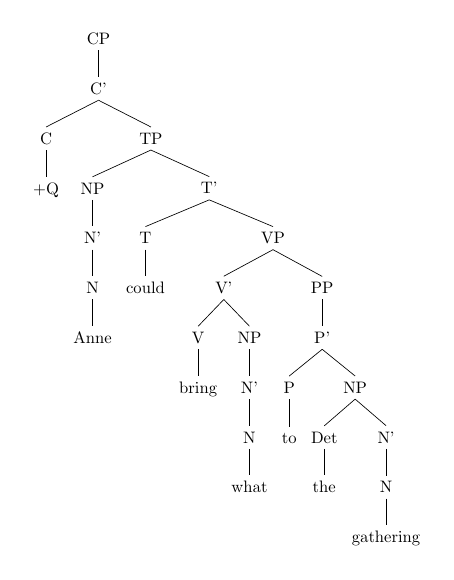
\begin{tikzpicture}[scale=0.6]
        \Tree [.CP [.C'
            [.C +Q ]
            [.TP
                [.NP [.N' [.N Anne ] ] ]
                [.T'
                    [.T could ]
                    [.VP
                        [.V'
                            [.V bring ]
                            [.NP [.N' [.N what ] ] ] ]
                        [.PP [.P'
                            [.P to ]
                            [.NP
                                [.Det the ]
                                [.N' [.N gathering ] ] ] ] ] ] ] ] ] ]
    \end{tikzpicture}
    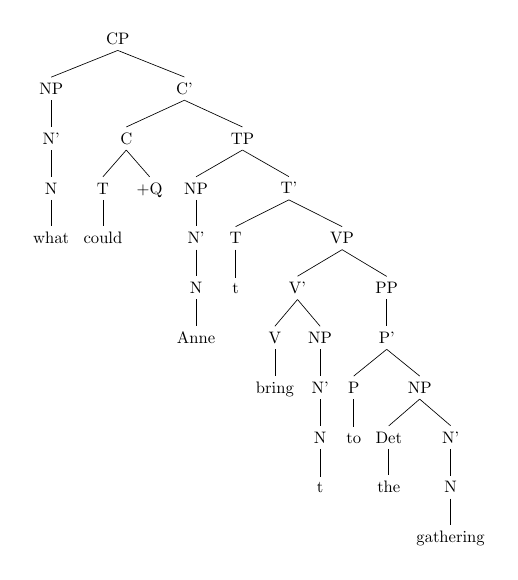
\begin{tikzpicture}[scale=0.6]
        \Tree [.CP
            [.NP [.N' [.N what ] ] ]
            [.C'
                [.C
                    [.T could ]
                    +Q ]
                [.TP
                    [.NP [.N' [.N Anne ] ] ]
                    [.T'
                        [.T t ]
                        [.VP
                            [.V'
                                [.V bring ]
                                [.NP [.N' [.N t ] ] ] ]
                            [.PP [.P'
                                [.P to ]
                                [.NP
                                    [.Det the ]
                                    [.N' [.N gathering ] ] ] ] ] ] ] ] ] ]
    \end{tikzpicture}
\end{center}

\section*{Chapter 5, Problem 13}

\tikzset{every picture/.style = {scale=0.55}}
\begin{multicols}{2}
    \begin{enumerate}[a)]
        \item The efficient workers finished very quickly.
        \begin{center}
            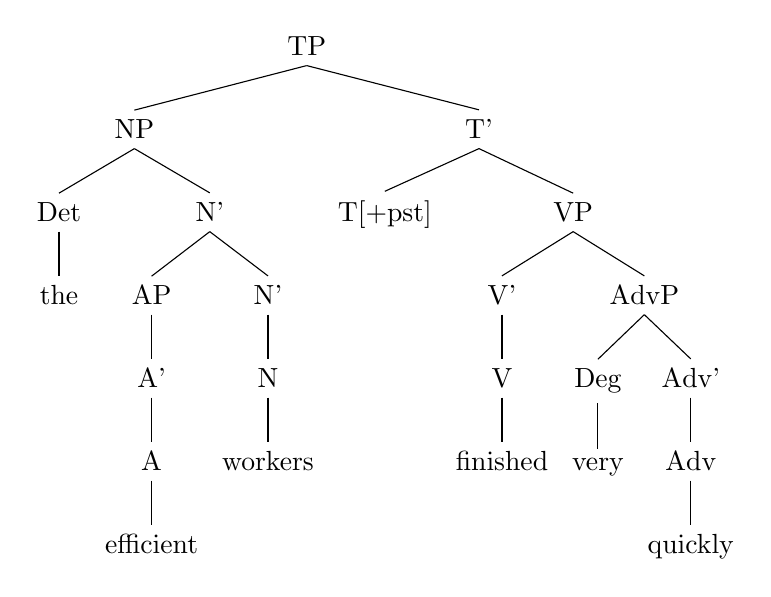
\begin{tikzpicture}
                \Tree [.TP
                    [.NP
                        [.Det the ]
                        [.N'
                            [.AP [.A' [.A efficient ] ] ]
                            [.N' [.N workers ] ] ] ]
                    [.T'
                        T[+pst]
                        [.VP
                            [.V' [.V finished ] ]
                            [.AdvP
                                [.Deg very ]
                                [.Adv' [.Adv quickly ] ] ] ] ] ]
            \end{tikzpicture}
        \end{center}
        \item A very clever engineer designed this new car.
        \begin{center}
            \begin{tikzpicture}[scale=0.90]
                \Tree [.TP
                    [.NP
                        [.Det a ]
                        [.N'
                            [.AP
                                [.Deg very ]
                                [.A' [.A clever ] ] ]
                            [.N' [.N engineer ] ] ] ]
                    [.T'
                        T[+pst]
                        [.VP [.V'
                            [.V designed ]
                            [.NP
                                [.Det this ]
                                [.N'
                                    [.AP [.A' [.A new ] ] ]
                                    [.N' [.N car ] ] ] ] ] ] ] ]
            \end{tikzpicture}
        \end{center}
        \columnbreak
        \item The large tiger suddenly leapt into the tree.
        \begin{center}
            \begin{tikzpicture}[scale=0.95]
                \Tree [.TP
                    [.NP
                        [.Det the ]
                        [.N'
                            [.AP [.A' [.A large ] ] ]
                            [.N' [.N tiger ] ] ] ]
                    [.T'
                        T[+pst]
                        [.VP
                            [.AdvP [.Adv' [.Adv suddenly ] ] ]
                            [.V'
                                [.V' [.V leapt ] ]
                                [.PP [.P'
                                    [.P into ]
                                    [.NP
                                        [.Det the ]
                                        [.N' [.N tree ] ] ] ] ] ] ] ] ]
            \end{tikzpicture}
        \end{center}
        \vfill\null
    \end{enumerate}
\end{multicols}

\pagebreak

\section*{Part II}

\tikzset{every picture/.style = {scale=0.8}}
\begin{multicols}{2}
    \begin{enumerate}
        \item The dogs had a snack.
        \begin{center}
            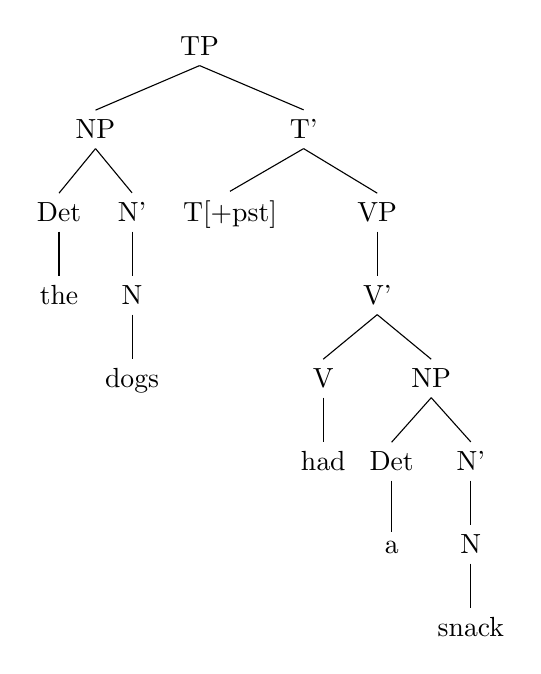
\begin{tikzpicture}
                \Tree [.TP
                    [.NP
                        [.Det the ]
                        [.N' [.N dogs ] ] ]
                    [.T'
                        T[+pst]
                        [.VP [.V'
                            [.V had ]
                            [.NP
                                [.Det a ]
                                [.N' [.N snack ] ] ] ] ] ] ]
            \end{tikzpicture}
        \end{center}
        \item A scientist will speak to the group tomorrow.
        \begin{center}
            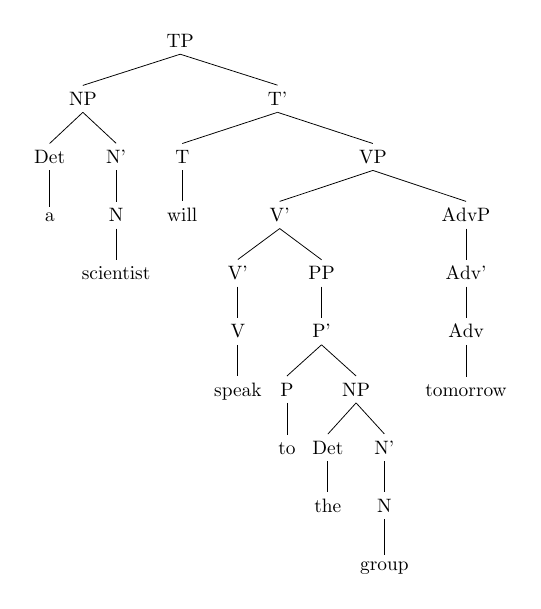
\begin{tikzpicture}[scale=0.7]
                \Tree [.TP
                    [.NP
                        [.Det a ]
                        [.N' [.N scientist ] ] ]
                    [.T'
                        [.T will ]
                        [.VP
                            [.V'
                                [.V' [.V speak ] ]
                                [.PP [.P'
                                    [.P to ]
                                    [.NP
                                        [.Det the ]
                                        [.N' [.N group ] ] ] ] ] ]
                            [.AdvP [.Adv' [.Adv tomorrow ] ] ] ] ] ]
            \end{tikzpicture}
        \end{center}
        \item The tall trees block the road.
        \begin{center}
            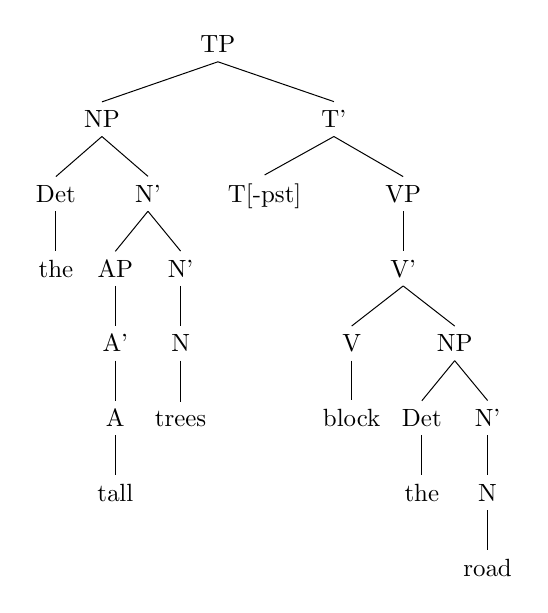
\begin{tikzpicture}[scale=0.9]
                \Tree [.TP
                    [.NP
                        [.Det the ]
                        [.N'
                            [.AP [.A' [.A tall ] ] ]
                            [.N' [.N trees ] ] ] ]
                    [.T'
                        T[-pst]
                        [.VP [.V'
                            [.V block ]
                            [.NP
                                [.Det the ]
                                [.N' [.N road ] ] ] ] ] ] ]
            \end{tikzpicture}
        \end{center}
        \item The peaches never appear ripe in winter.
        \begin{center}
            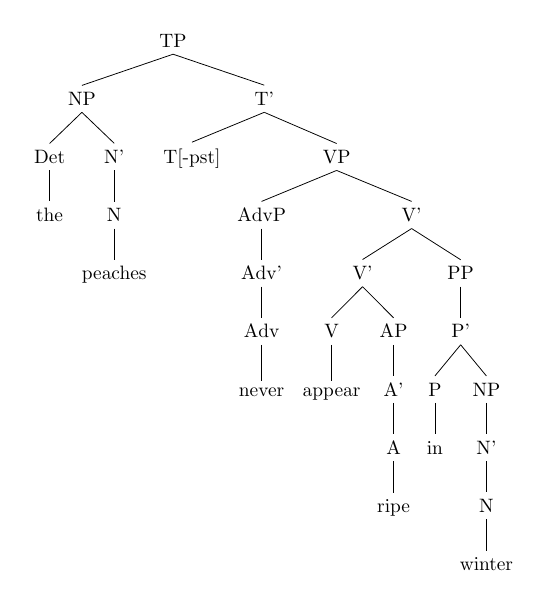
\begin{tikzpicture}[scale=0.7]
                \Tree [.TP
                    [.NP
                        [.Det the ]
                        [.N' [.N peaches ] ] ]
                    [.T'
                        T[-pst]
                        [.VP
                            [.AdvP [.Adv' [.Adv never ] ] ]
                            [.V'
                                [.V'
                                    [.V appear ]
                                    [.AP [.A' [.A ripe ] ] ] ]
                                [.PP [.P'
                                    [.P in ]
                                    [.NP [.N' [.N winter ] ] ] ] ] ] ] ] ]
            \end{tikzpicture}
        \end{center}
    \end{enumerate}
\end{multicols}
\begin{enumerate}
    \setcounter{enumi}{4}
    \item My friend had colorful pictures of her family
    \begin{center}
        \begin{tikzpicture}[scale=0.8]
            \Tree [.TP
                [.NP
                    [.AP [.A' [.A my ] ] ]
                    [.N' [.N friend ] ] ]
                [.T'
                    T[+pst]
                    [.VP [.V'
                        [.V had ]
                        [.NP
                            [.AP [.A' [.A colorful ] ] ]
                            [.N'
                                [.N pictures ]
                                [.PP [.P'
                                    [.P of ]
                                    [.NP
                                        [.AP [.A' [.A her ] ] ]
                                        [.N' [.N family ] ] ] ] ] ] ] ] ] ] ]
        \end{tikzpicture}
    \end{center}
    \item The burglar threatened the student with a knife.
    \begin{center}
        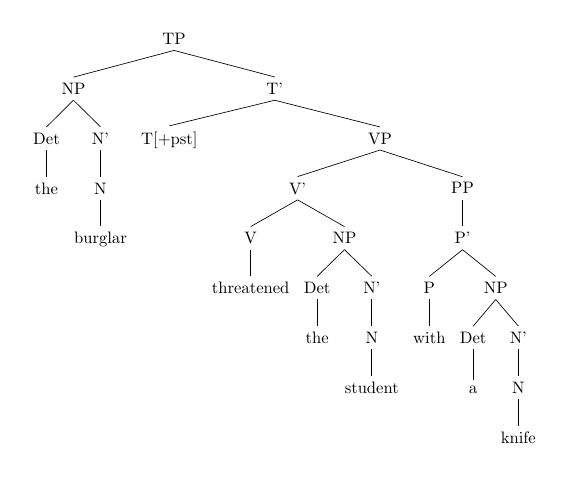
\begin{tikzpicture}[scale=0.6]
            \Tree [.TP
                [.NP
                    [.Det the ]
                    [.N' [.N burglar ] ] ]
                [.T'
                    T[+pst]
                    [.VP
                        [.V'
                            [.V threatened ]
                            [.NP
                                [.Det the ]
                                [.N' [.N student ] ] ] ]
                        [.PP [.P'
                            [.P with ]
                            [.NP
                                [.Det a ]
                                [.N' [.N knife ] ] ] ] ] ] ] ]
        \end{tikzpicture}
        \begin{tikzpicture}[scale=0.6]
            \Tree [.TP
                [.NP
                    [.Det the ]
                    [.N' [.N burglar ] ] ]
                [.T'
                    T[+pst]
                    [.VP [.V'
                        [.V threatened ]
                        [.NP
                            [.Det the ]
                            [.N'
                                [.N student ]
                                [.PP [.P'
                                    [.P with ]
                                    [.NP
                                        [.Det a ]
                                        [.N' [.N knife ] ] ] ] ] ] ] ] ] ] ]

        \end{tikzpicture}
    \end{center}
    The left interpretation means that the burglar has the knife and uses it to threaten the student, while the right interpretation
    means that the student has the knife and the burglar threatens that student.
    \item I shot an elephant in my pajamas.
    \begin{center}
        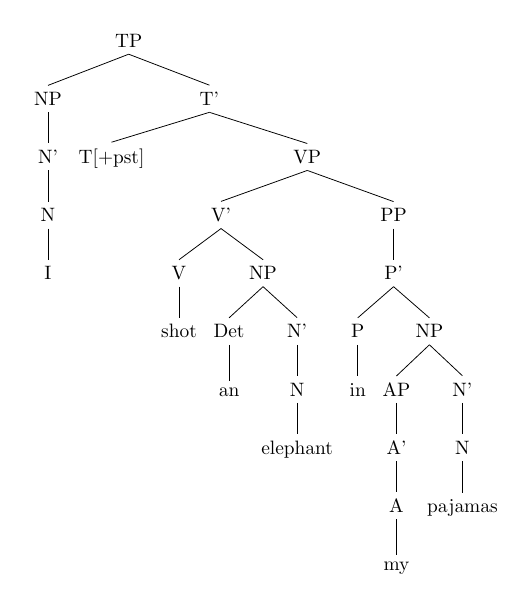
\begin{tikzpicture}[scale=0.7]
            \Tree [.TP
                [.NP [.N' [.N I ] ] ]
                [.T'
                    T[+pst]
                    [.VP
                        [.V'
                            [.V shot ]
                            [.NP
                                [.Det an ]
                                [.N' [.N elephant ] ] ] ]
                        [.PP [.P'
                            [.P in ]
                            [.NP
                                [.AP [.A' [.A my ] ] ]
                                [.N' [.N pajamas ] ] ] ] ] ] ] ]
        \end{tikzpicture}
        \begin{tikzpicture}[scale=0.7]
            \Tree [.TP
                [.NP [.N' [.N I ] ] ]
                [.T'
                    T[+pst]
                    [.VP
                        [.V'
                            [.V shot ]
                            [.NP
                                [.Det an ]
                                [.N'
                                    [.N elephant ]
                                    [.PP [.P'
                                        [.P in ]
                                        [.NP
                                            [.AP [.A' [.A my ] ] ]
                                            [.N' [.N pajamas ] ] ] ] ] ] ] ] ] ] ]
        \end{tikzpicture}
    \end{center}
    The left interpretation means that the speaker made the shot while the speaker was inside the pajamas, while the right interpretation means
    that the speaker made the shot at an elephant that was inside the pajamas.
\end{enumerate}

\end{document}